% !TEX program = xelatex
\documentclass[12pt,a4paper]{ctexart}

% ---------- Packages ----------
\usepackage{amsmath,amssymb,amsfonts}
\usepackage{graphicx}
\usepackage{algorithm,algorithmic}
\usepackage{url}
\usepackage{hyperref}
\hypersetup{hidelinks=true}
\usepackage{textcomp}
\usepackage{cleveref}
\usepackage{booktabs}
\usepackage{subcaption}
\usepackage{comment}
\usepackage{float}
\usepackage{bm}
\usepackage{multirow}
\usepackage{caption}
\captionsetup[figure]{font=small}
\captionsetup[table]{font=small}

% Adjust spacing
\setlength{\abovedisplayskip}{5pt plus 1pt minus 1pt}
\setlength{\belowdisplayskip}{5pt plus 1pt minus 1pt}
\setlength{\abovedisplayshortskip}{2pt plus 1pt minus 1pt}
\setlength{\belowdisplayshortskip}{2pt plus 1pt minus 1pt}

% ---------- Theorem Environments ----------
\let\proof\relax
\let\endproof\relax
\usepackage{amsthm}
\usepackage{etoolbox}
\AtEndEnvironment{proof}{\hfill$\blacksquare$}

\theoremstyle{plain}
\newtheorem{theorem}{定理}[section]
\newtheorem{lemma}[theorem]{引理}
\newtheorem{proposition}[theorem]{命题}
\newtheorem{corollary}[theorem]{推论}

\theoremstyle{definition}
\newtheorem{definition}[theorem]{定义}
\newtheorem{assumption}[theorem]{假设}
\newtheorem{example}[theorem]{例}

\theoremstyle{remark}
\newtheorem{remark}[theorem]{注记}
\newtheorem{note}[theorem]{注}

\crefname{assumption}{假设}{假设}
\Crefname{assumption}{假设}{假设}
\crefname{theorem}{定理}{定理}
\Crefname{theorem}{定理}{定理}
\crefname{equation}{式}{式}

\renewcommand{\qedsymbol}{$\blacksquare$}

% Custom commands
\newcommand{\define}{\mathrel{\mathop:}=}

\begin{document}

\title{基于Koopman的绳驱空间机械臂数据驱动建模与控制}
\author{作者一\thanks{作者单位，城市，国家。} \and 作者二 \and 作者三}

\maketitle

\begin{abstract}


1、本文




\end{abstract}

\noindent\textbf{关键词：}绳驱空间机械臂；Koopman 算子；数据驱动建模；深度 Koopman；模型预测控制；闭环轨迹跟踪

% ---------- 正文 ----------
\section{引言}
\label{sec:introduction}
这睡觉哦自己鞥文明\cite{huangImprovingRobustnessOutofDistribution2025}


\begin{figure}[htbp]
  \centering
  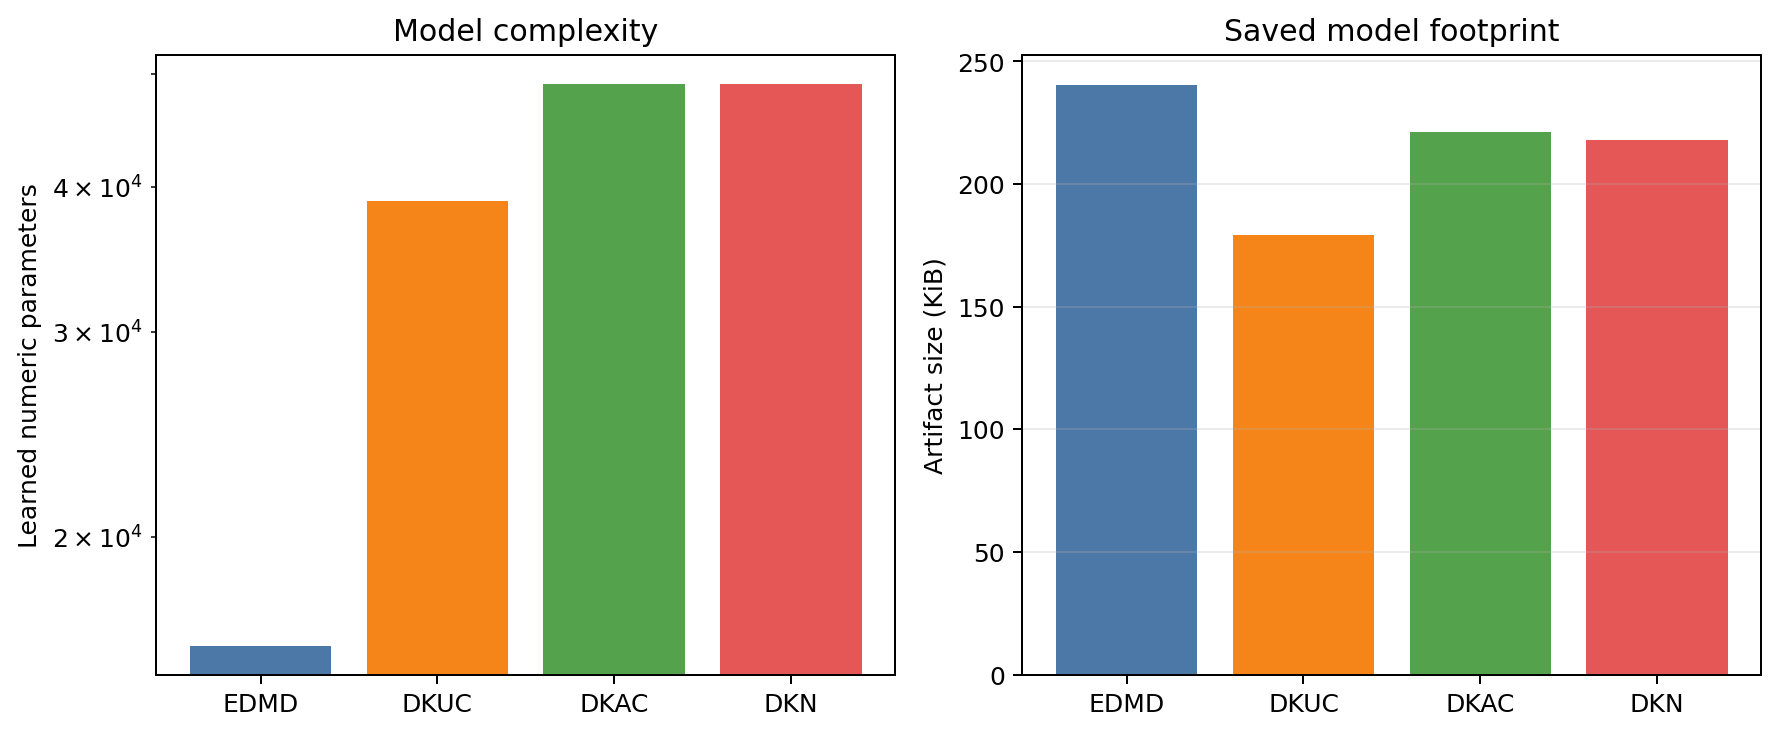
\includegraphics[width=0.8\linewidth]{figure/model_complexity_comparison.png}
  \caption{我们的方法概览}
  \label{fig:overview}
\end{figure}

% TODO: 在这里写引言。

\section{相关工作}
\label{sec:related}

% TODO: 在这里写相关工作。

\section{预备知识}
\label{sec:preliminary}

% TODO: 在这里写预备知识。

\section{理论分析}
\label{sec:theory}

% TODO: 在这里写理论分析。

\section{方法}
\label{sec:method}

% TODO: 在这里写方法。

\section{实验}
\label{sec:experiment}

% TODO: 在这里写实验。

\section{结论}
\label{sec:conclusion}

% TODO: 在这里写结论。

\section*{致谢}

% TODO: 在这里写致谢。


% ---------- 参考文献 ----------
\bibliographystyle{unsrt}
\bibliography{reference.bib}

% ---------- 附录 ----------
% \appendix
% \section{附录}

% TODO: 在这里写附录。


\end{document}
